% MaCVi 2027 Diver3D challenge: team report (WACV 2027 author kit, camera-ready layout with page numbers)
\documentclass[10pt,twocolumn,letterpaper]{article}
\usepackage[pagenumbers]{wacv}
%
% --- inline annotations
%
\newcommand{\red}[1]{{\color{red}#1}}
\newcommand{\todo}[1]{{\color{red}#1}}
\newcommand{\TODO}[1]{\textbf{\color{red}[TODO: #1]}}
% --- disable by uncommenting  
% \renewcommand{\TODO}[1]{}
% \renewcommand{\todo}[1]{#1}



\renewcommand{\ttdefault}{cmtt}
\definecolor{wacvblue}{rgb}{0.21,0.49,0.74}
\usepackage[pagebackref,breaklinks,colorlinks,allcolors=wacvblue]{hyperref}

\def\wacvPaperID{*****}
\def\confName{WACV}
\def\confYear{2027}

\newcommand{\sds}{\mbox{SDS}}
\newcommand{\aoe}{\mbox{AOE\textsubscript{3D}}}
\newcommand{\apt}[1]{\mbox{AP\textsubscript{3D}@#1}}
\newcommand{\apb}[1]{\mbox{AP\textsubscript{BEV}@#1}}

\title{Team FAU CAAI at the MaCVi 2027 Diver3D Challenge:\\A Voxel CenterPoint Ensemble and What the Benchmark Taught Us}

\author{Dan Zimmerman \qquad George Sklivanitis\\
Center for Connected Autonomy and AI, Florida Atlantic University\\
Boca Raton, FL, USA}

\begin{document}
\maketitle

\begin{abstract}
We describe the FAU CAAI entry to the MaCVi 2027 Diver3D challenge, which asks for 9-DoF diver boxes with full SO(3) orientation from 3D imaging-sonar frames.
Our system reimplements the dense SonarVoxNet baseline with finer height voxels and a rotation loss folded over the front--back symmetry of the cuboid.
Detector weights are trained on the train split only; validation selected checkpoints and inference settings.
Nine models, some with three-frame inputs, are fused with mirror and radial-scale test-time augmentation, weighted box fusion in SO(3), and non-causal per-recording track smoothing.
Our best entry scores \sds{} 0.7290 on the hidden test set and ranks fourth of four teams.
Its gap to the winner comes from mAP\textsubscript{3D}; on matched boxes, its translation (0.163\,m) and orientation (27.4\textdegree) errors are lower than those of every entry ranked above it.
Over more than 80 training runs and thirteen uploads we also made measurements of the benchmark as seen through our pipeline.
Validation ranks our ensembles but over-predicts test by 0.017--0.039 \sds{}.
For matched validation boxes, after adjusting for range and body orientation, labelled widths show recording offsets of up to $\pm$40\% relative to the model reference, against at most 10\% for our predictions.
Confident detections persist through long unlabelled stretches at the position of the last labelled diver.
In our pipeline, greedy bird's-eye-view non-maximum suppression at IoU 0.1 suppressed close diver pairs.
We also list what did not help, so that others need not repeat it.
\end{abstract}

\section{Introduction}
Diver3D~\cite{sonarvoxnet2026} is built from the uScenes campaign~\cite{uscenes2026}: 36 recordings and 37{,}010 sonar frames with 9-DoF diver boxes, split 21/7/8 into train, validation and hidden test.
Each frame is a point cloud with at most one return per beam on a 256$\times$64 beam grid spanning $\pm$45\textdegree{} in bearing and $\pm$20\textdegree{} in elevation.
Entries are ranked by the Sonar--Diver Detection Score
\begin{equation}
\begin{split}
\sds = \tfrac{1}{6}\big[\,&3\,\mathrm{mAP_{3D}} + (1-\mathrm{ATE})\\
&+ (1-\mathrm{ASE}) + (1-\aoe/90^\circ)\big],
\end{split}
\end{equation}
where mAP\textsubscript{3D} averages AP\textsubscript{3D} over 3D IoU thresholds 0.30, 0.35 and 0.40.
This report summarises our submitted system and the development experiments behind it, several of which concern the benchmark rather than our model.

\section{System}
\label{sec:system}
\paragraph{Detector.}
We reimplemented the dense SonarVoxNet variant~\cite{sonarvoxnet2026}.
Points inside $[0,12]\times[-5,5]\times[-2.5,2.5]$\,m are voxelised at $0.1\times0.1\times0.25$\,m.
A dynamic voxel feature encoder~\cite{voxelnet2018} (two linear layers with 64 and 128 channels, max-pooled per voxel) sees each point's coordinates, intensity, offsets to the voxel mean and centre, and, for three-frame members, a frame-offset channel.
These members stack the two previous frames of the same recording without motion compensation.
3D convolutions collapse the 20 height bins into a bird's-eye-view (BEV) map.
A 2D neck (128 channels, 4/6/6 residual blocks, upsampled to 256 channels at output stride 2) feeds a CenterPoint head~\cite{centerpoint2021}.
The head predicts a Gaussian focal heat map (minimum overlap 0.7, radius at least one cell, $\alpha=2$, $\beta=4$) and regresses centre offset, height, log extents and a continuous 6D rotation~\cite{zhou2019continuity} decoded by Gram--Schmidt, with unit loss weights.
Because the cuboid maps onto itself under a half-turn about its up axis, the L1 rotation loss takes the minimum over the two equivalent targets.
The model has 9.4\,M parameters.

\paragraph{Differences from the published baseline.}
Height voxels are 0.25\,m instead of 0.5\,m, our largest single gain: validation \sds{} 0.679 against 0.640 over two runs each, and the five reference seeds of member 5's configuration, also at 0.25\,m, average 0.670.
The rotation loss is folded over the half-turn symmetry, which the metric also folds; we did not ablate this.
Detections are kept down to score 0.05 instead of 0.30, because AP integrates over recall.
Our smoothing uses fixed centred windows in place of the published causal refinement, which uses learned residual regressors; our validation-fitted reimplementation of those regressors did not transfer across recordings.

\paragraph{Training.}
All detector weights are trained on the train split only: 20 epochs, batch 8, AdamW (learning rate $10^{-3}$, weight decay 0.01, one-cycle schedule), gradient clipping at 35, about 1.4\,h on one H200.
Augmentation is a $y$-mirror, small rotations ($\pm$5\textdegree{} yaw and roll, $\pm$3\textdegree{} pitch), up to 15\% point dropout, 10\% intensity jitter, and copy-paste~\cite{second2018} of real diver returns cropped from train labels (at least 20 points), placed within $\pm$40\textdegree{} of bearing with $\pm$8\textdegree{} elevation jitter and range scaled by 0.85--1.15.
Pasting starts at four divers per frame and anneals by one per epoch to a floor of zero or one, beginning at 45\% or 65\% of training; two members paste beam-consistently, so that each pasted diver occludes the beams behind it.
Checkpoints are the best validation \sds{} from the epoch at which pasting reaches its floor; for floor-zero members, that is the first epoch in which empty training frames carry no pasted divers.

\paragraph{Inference.}
The nine members (\cref{tab:members}) run on each cloud and on its $y$-mirror; for the best entry they also run on the cloud scaled radially by 1.05, with boxes scaled back, giving 36 passes.
Each pass keeps the top 100 heat-map peaks and applies greedy BEV non-maximum suppression (NMS) at IoU 0.1.
Weighted box fusion~\cite{wbf2021} merges the passes in SO(3): clusters form at 3D IoU $>0.3$, centre and extents are score-weighted means, rotation is the weighted chordal mean after resolving the half-turn ambiguity, and the score is the sum over passes divided by the number of passes.
Within each recording, boxes are linked into tracks by BEV IoU $\ge 0.2$ and smoothed over centred windows of $\pm$1 frame for the centre, $\pm$5 for rotation and $\pm$8 for extents; scores are unchanged and no box is added or removed.
Because the windows are centred, smoothing is non-causal: it uses up to eight frames before and after each frame of the same test recording, inputs only, with no learning on test data.
Detections below 0.05 are dropped; the best entry has 15{,}072 boxes over 8{,}112 frames.
Validation selected the checkpoints, the members and every post-processing setting: NMS and fusion thresholds, smoothing windows, score cut and scale factor.
Measured one at a time on validation, mirror augmentation added about 0.02 \sds{} to a single model, ensembling about 0.03, smoothing 0.009--0.010 on our ensembles and the radial scale 0.005 (0.0013 on test); the gains are not additive.
Each set of 18 passes over the test set took about 22 minutes on one shared H200.
We used no external data, pretrained weights or camera imagery.
All thirteen uploads are listed in \cref{tab:uploads}; our standing entry is the best-scoring one.
One upload (\texttt{a45x7}) chose members for near-range recall on validation, motivated by the range profile of our own test predictions, and one (\texttt{ens9-top1}) was a diagnostic of the test set.

\begin{table}[t]
\centering
\footnotesize
\setlength{\tabcolsep}{3pt}
\begin{tabular}{@{}cccccl@{}}
\toprule
\# & Frames & Floor / start & Paste & Epoch & Val \sds{} \\
\midrule
1, 2 & 1 & 1 / 0.65 & plain & 16, 15 & 0.683, 0.674 \\
3 & 3 & 1 / 0.65 & plain & 15 & 0.700 \\
4 & 1 & 0 / 0.65 & plain & 16 & 0.675 \\
5--7 & 3 & 0 / 0.45 & plain & 12--15 & 0.693, 0.655, 0.670 \\
8, 9 & 3 & 0 / 0.45 & occluding & 13, 12 & 0.671, 0.652 \\
\bottomrule
\end{tabular}
\caption{Ensemble members. Frames: current frame only (1) or with the two previous frames stacked (3). Floor / start: paste floor and the fraction of training at which annealing starts. Val \sds{}: single model, without test-time augmentation or smoothing. Rows with several members differ only in the seed.}
\label{tab:members}
\end{table}

\section{Results}
\label{sec:results}
\Cref{tab:uploads} lists our uploads.
The best, \texttt{d3-vz-ens9-sc105}, scores \sds{} 0.7290 on test with mAP\textsubscript{3D} 0.717, \apt{0.35} 0.729, \apt{0.50} 0.407, \apb{0.35} 0.832, ATE 0.163\,m, ASE 0.309 and \aoe{} 27.4\textdegree.
On the public leaderboard of 24 October 2026~\cite{macvilb2026}, every entry ranked above it has ATE $\ge$ 0.165\,m and \aoe{} $\ge$ 29.6\textdegree; both are computed on matched detections only.
Against the top entry (0.7588), mAP\textsubscript{3D} (0.788) and ASE (0.302) account for 0.036 and 0.001 of the gap, while our ATE and \aoe{} recover 0.001 and 0.006.
That entry's \apb{0.35} is 0.891 against our 0.832, while its \apt{0.50} (0.418) is close to ours.

The SonarVoxNet paper reports test \sds{} 0.673 for its single model (mAP\textsubscript{3D} 0.690, \aoe{} 46.2\textdegree) and 0.719 with causal refinement, computed before the challenge scorer was released~\cite{sonarvoxnet2026}.
Our single-model pipeline (member 5 with mirror augmentation and non-causal smoothing) scores 0.6954 on test, with lower mAP\textsubscript{3D} (0.662) and much lower \aoe{} (27.9\textdegree).
Our best ensemble is numerically 0.010 above the refined baseline; the scorers differ and our smoothing is non-causal, so this is not a like-for-like comparison.

\begin{table}[t]
\centering
\footnotesize
\setlength{\tabcolsep}{3pt}
\begin{tabular}{@{}llcc@{}}
\toprule
Entry (\texttt{d3-vz-}) & Members and change & Val & Test \\
\midrule
\texttt{ens3-ref} & 3 single-frame models & 0.7405 & 0.7235 \\
\texttt{ens7-ref} & members 1--7 & 0.7550 & 0.7264 \\
\texttt{fp6} & 6 models chosen for few FPs & 0.7485 & 0.7217 \\
\texttt{ens7-s2} & 1--7 + refiner trained on train & 0.7581 & 0.7246 \\
\texttt{single-ref} & member 5 alone & 0.7320 & 0.6954 \\
\texttt{ens9-occl} & members 1--9 & 0.7541 & 0.7277 \\
\texttt{ens13-occl} & 1--7 + 6 occluding-paste models & 0.7543 & 0.7229 \\
\texttt{occl8} & 8 occluding-paste models & 0.7448 & 0.7145 \\
\texttt{ens9-calib} & 1--9 + correction fitted on val & -- & 0.7207 \\
\texttt{last6} & 6 last-epoch checkpoints & 0.7361 & 0.6973 \\
\texttt{a45x7} & 7 models chosen for near recall & 0.7508 & 0.7137 \\
\texttt{ens9-sc105} & 1--9 + radial scale 1.05 & 0.7599$^*$ & \textbf{0.7290} \\
\texttt{ens9-top1} & 1--9, top box per frame only & 0.6832$^*$ & 0.6241 \\
\bottomrule
\end{tabular}
\caption{Our uploads. All include mirror augmentation, fusion and smoothing. $^*$Validation value of the same recipe on members 1--7.}
\label{tab:uploads}
\end{table}

\begin{figure*}[t]
\centering
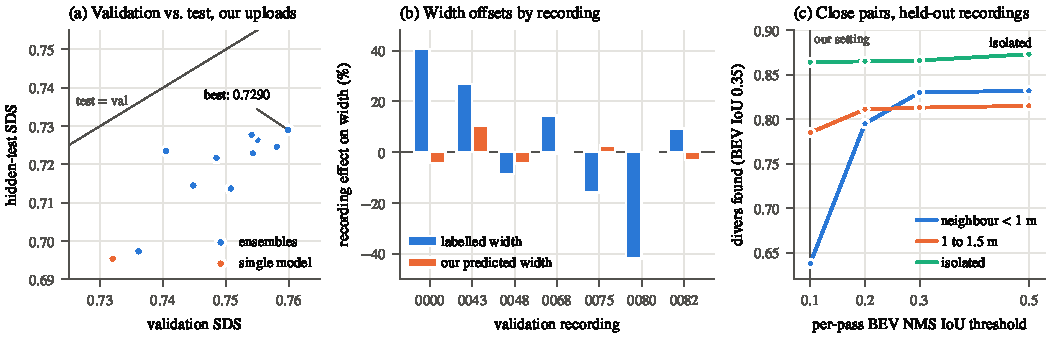
\includegraphics[width=\textwidth]{fig/overview.pdf}
\caption{(a) Validation against hidden-test \sds{} for our uploads with a validation counterpart. (b) Recording effects on box width in validation, from a mixed-effects model of log width with range and body orientation relative to the beam as covariates: relative to the model reference, labelled widths shift by $-42$\% to $+40$\% between recordings, our predictions by at most about 10\%. (c) Fraction of labelled divers found at BEV IoU 0.35 on 14 train recordings held out from two fold detectors, after fusion and smoothing, as the per-pass NMS threshold rises.}
\label{fig:overview}
\end{figure*}

\section{Observations on the benchmark}
\label{sec:lessons}
\paragraph{Validation ranks entries but over-predicts test.}
For the eleven uploads with a validation counterpart, test is lower by 0.017--0.039 \sds{} (mean 0.031; \cref{fig:overview}a); for \texttt{ens9-sc105} the counterpart is its seven-member proxy.
The drop does not scale with the validation score ($r=-0.14$).
The largest drop (0.039) belongs to an ensemble of last-epoch checkpoints chosen without validation, so best-epoch selection does not explain it, although one such entry cannot exclude a smaller selection component.
Validation ranks our ensembles moderately well (Spearman 0.75, $n=10$, bootstrap 95\% interval 0.2--0.96; the uploads share members), but the residual scatter of about 0.005 means differences of a few thousandths did not survive.
The refiner gained 0.003 on validation and lost 0.002 on test, and the validation-fitted correction lost 0.007 on test.
Single models of one configuration have a seed standard deviation of 0.015 (0.655--0.693 over five seeds).
Resolving a 0.02 difference at 80\% power therefore needs about ten seeds per arm, and two seeds against our five-seed reference resolve only differences of about 0.04.
From mid-October we wrote paired acceptance criteria into our results log before each run, and we treat two-seed comparisons as screening only.
Lower-ranked boxes matter more on test: keeping only the top-scoring box per frame costs 0.104 \sds{} on test (nine members) against 0.072 on validation (seven members), consistent with more divers per occupied frame or a different score ordering.

\paragraph{Box widths differ between recordings.}
For validation boxes matched by our ensemble (the best 3D-overlap prediction for each labelled box), we fitted a mixed-effects model of $\log(\text{predicted}/\text{labelled width})$.
The recording is a random intercept; range, log range and the vertical and along-beam components of the body axis are fixed effects.
Recording indicators explain 64\% of the variance left by the covariates (partial $R^2$, seven recordings).
Fitted to each side separately, the recording effects have standard deviation 0.30 for log labelled width and 0.05 for log predicted width, and the two sets of effects are uncorrelated ($r=0.04$; \cref{fig:overview}b).
We cannot tell whether these offsets reflect annotation practice or real differences between divers and equipment, and seven recordings are few for a variance estimate.
As label-informed sensitivities, not achievable gains: substituting labelled extents for predicted ones would add 0.072 validation \sds{}, of which 0.032 comes from each track's mean extent.
Validation-fitted, point-conditioned residual regressors did not survive leave-one-recording-out, and a track-level size prior learned on the 21 train recordings added 0.001.

\paragraph{Detections persist through unlabelled stretches.}
26\% of train and validation frames carry no box.
As a label-informed sensitivity, removing all detections in those frames, and those with no overlap with any labelled diver, would add 0.059 \apt{0.35} on validation.
Some of them sit on the returns of a previously labelled diver.
In recording 0075, a labelled diver's returns stay in place, and keep being detected, through 651 unlabelled frames, and the next label falls on the same returns.
At 19 of 72 label-to-no-label transitions on validation, a detection with mean score at least 0.3 over the next five frames continues within 0.5\,m of the diver's last labelled position.
Keeping half of the unlabelled training frames free of pasted divers, so that the network sees them as negatives, did not reduce false positives at matched recall; with one curriculum it increased them$^\dagger$.

\paragraph{In our pipeline, greedy NMS suppressed close diver pairs.}
2.6\% of training divers have another diver within 1\,m.
Under 2\,m our median predicted BEV footprint is 1.5--1.6 times the labelled one in area (about 1.0 beyond 2\,m), so a buddy beside a diver can overlap its box by more than the per-pass NMS threshold of 0.1 and be discarded.
We tested this on 14 train recordings held out from two fold detectors.
Raising the threshold to 0.3 lifts BEV recall from 0.64 to 0.83 for divers with a neighbour within 1\,m and from 0.79 to 0.81 for those with one at 1--1.5\,m; for isolated divers it moves from 0.864 to 0.866 (\cref{fig:overview}c).
In the two pair-heavy recordings, the share of close pairs with both divers matched one-to-one rises from 0.53 to 0.88 and from 0.42 to 0.73.
Their \sds{} rises by 0.017 and 0.007 (block-bootstrap 95\% intervals over frames 0.001--0.049 and 0.002--0.011), against at most 0.0025 in the nine pair-free recordings with labels; validation, with 20 close-pair boxes, is unchanged (0.7550).
No two detections with score at least 0.3 in our test output lie within 1\,m of each other.
Rerunning at 0.3 adds 652 mostly low-scoring boxes, but only 4 confident ones 0.35--1.2\,m from an existing detection in 8{,}112 frames.
Without labels we cannot tell whether close pairs are scarce in the test set or lost earlier in our pipeline, so we did not rely on the change.

\paragraph{What did not help.}
\Cref{tab:negative} lists the changes that did not meet their criteria.
These screening runs, mostly of one or two seeds, gave no evidence of improvement; the better vertical-attention seed (0.687) was not matched by the other (0.654).
Only the range-view branch alone was clearly worse (0.610, outside the range of every reference seed).
Local-structure features and beam-grid dropout were 0.023--0.027 below the reference mean, at the edge of what two seeds can resolve.
Several changes lowered near-range recall, which matters here.
By our own test predictions, not labels, 57\% of test frames come from three recordings whose detected divers sit at a median range of 1.9--2.3\,m.
The nine occluding-paste models whose near-range recall we measured reached 0.57--0.65, against 0.64--0.72 (mean 0.68) for five plain-paste seeds$^\dagger$.

\begin{table}[t]
\centering
\footnotesize
\setlength{\tabcolsep}{2pt}
\begin{tabular}{@{}lr@{}}
\toprule
Change (seeds or models) & Val \sds{} or effect \\
\midrule
\multicolumn{2}{@{}l}{\emph{Representation}} \\
Polar (range $\times$ bearing) BEV grid$^\ddagger$ (2) & 0.639, 0.650 \\
Range-view branch, alone / fused~\cite{rangedet2021} (1+1) & 0.610 / 0.651 \\
Ray-cast visibility channels~\cite{wysiwyg2020} (1) & 0.652 \\
Vertical attention over height bins~\cite{rtnhplus2023}$^\dagger$ (2) & 0.654, 0.687 \\
Local point structure instead of xyz~\cite{gblobs2025} (2) & 0.649, 0.637 \\
\multicolumn{2}{@{}l}{\emph{Losses and heads}} \\
Vertical-position classification head (2) & 0.678, 0.651 \\
Gaussian box KL loss~\cite{yang2022gaussian}$^\dagger$ (2) & 0.646, 0.651 \\
Uncertainty-weighted rotation loss$^\dagger$ (2) & 0.633, 0.668 \\
Larger heat-map positives~\cite{hotspots2020} (4) & mean 0.663 \\
\multicolumn{2}{@{}l}{\emph{Augmentation and data}} \\
Beam-occluding paste (8 models) & 0.652--0.684, mean 0.663 \\
Near-range paste, $1/r^2$ density$^\dagger$ (4) & near recall 0.55--0.58 \\
Whole-frame radial scaling (2) & 0.661, 0.674 \\
Beam-grid density dropout~\cite{lidardistill2022} (2) & 0.651, 0.641 \\
Unlabelled frames kept paste-free$^\dagger$ (2) & 0.662, 0.646 \\
Oversampling test-like recordings$^\ddagger$ (2 variants) & 0.640, 0.639 \\
\multicolumn{2}{@{}l}{\emph{Post-processing (on the ensemble)}} \\
Second-stage refiner trained on train & val $+$0.003, test $-$0.002 \\
Kalman / RTS smoother~\cite{barshalom2001} & no gain over window \\
Background-staticness rescoring~\cite{cfc2022} & AP\textsubscript{BEV} $\le-$0.025 \\
Medoid / median / min-extent fusion & below mean fusion \\
\bottomrule
\end{tabular}
\caption{Changes that did not meet their acceptance criteria; from mid-October, criteria were written into our results log before each run. Single-model values are validation \sds{} of each selected checkpoint, against a reference of 0.670 $\pm$ 0.015 (mean $\pm$ s.d., five seeds of member 5's configuration; 95\% interval 0.651--0.688). $^\ddagger$Built on the anneal-0.65 configuration, whose two seeds scored 0.665 and 0.642. Near recall: fraction of divers under 2\,m found at 3D IoU 0.35, reference 0.68. The occluding-paste row mixes three configurations. The rotation loss left \aoe{} unchanged. $^\dagger$Runs lost in a storage rollback; values are from our logged outputs.}
\label{tab:negative}
\end{table}

\section{Suggestions for the benchmark}
\label{sec:suggestions}
\textbf{Per-recording AP.}
For one of our validation ensembles, pooled \apb{0.35} is 0.861 against 0.879 for the box-weighted mean of per-recording values.
The pooled metric therefore also depends on how scores compare across recordings; reporting per-recording AP alongside it would expose that heterogeneity.

\textbf{Ignore regions.}
Where the organisers confirm divers in unlabelled stretches, an explicit ignore policy for them would clarify evaluation.

\textbf{Extent convention.}
A short note on what the box extents include, for example fins and equipment, would let entrants match it.

\section{Conclusion}
We hope the observations in \cref{sec:lessons}, on validation transfer, recording-dependent widths, detections in unlabelled stretches and close pairs, are useful for the challenge summary.
Code and logs are available on request; runs marked $\dagger$ were lost in a storage rollback.

{
    \small\raggedright
    \bibliographystyle{ieeenat_fullname}
    \bibliography{main}
}

\end{document}
